\ifx\wholebook\relax \else

\documentclass[b5paper]{article}
\usepackage[nomarginpar
  %, margin=.5in
]{geometry}

\addtolength{\oddsidemargin}{-0.05in}
\addtolength{\evensidemargin}{-0.05in}
\addtolength{\textwidth}{0.1in}

\usepackage[en]{../../../prelude}

\setcounter{page}{1}

\begin{document}

\title{Binary Search Tree: the `hello world' data structure}

\author{Larry~LIU~Xinyu
\thanks{{\bfseries Larry LIU Xinyu } \newline
  Email: liuxinyu95@gmail.com \newline}
  }

\maketitle
\fi

\markboth{Binary search tree}{Elementary Algorithms}

\ifx\wholebook\relax
\chapter{Binary Search Tree, the `hello world' data structure}
\numberwithin{Exercise}{chapter}
\fi

% ================================================================
%                 Introduction
% ================================================================
\section{Introduction}
\label{introduction} \index{binary search tree}

Array or list are typically considered the `hello world' data structures. However, we'll see they are not necessarily easy to implement in chapter 11. Upon imperative settings, array is the most elementary data structures. It is possible to implement linked-list using arrays (section  10.3 in \cite{CLRS}). While in functional settings, linked-list acts as the building blocks to create array and other data structures.

We start from Binary Search Trees (BST) as the `hello world' data structure. Let us see an interesting programming problem given by Bentley in {\em Programming Pearls}\cite{Bentley}. It is about to count the number of words in text. Here is an example solution:\index{word counter}

\lstset{language=C++, frame=single}
\begin{lstlisting}
int main(int, char**) {
    map<string, int> dict;
    string s;
    while (cin >> s)
        ++dict[s];
    for(auto it = dict.begin(); it != dict.end(); ++it)
        cout << it->first << ": " << it->second << "\n";
}
\end{lstlisting}

We can run it to count the words in a text file:

\begin{verbatim}
$ cat bbe.txt | ./wordcount > wc.txt
\end{verbatim}

The map provided in library is a kind of balanced binary search tree. Here we use the word as the key, and its occurrence number as the value. This program runs fast, which reflects the power of binary search tree. Before dive into it, let us first see the more generic tree, the binary tree. A binary tree can be defined recursively. It is

\index{binary tree}

\begin{itemize}
\item either empty;
\item or contains 3 parts: the key, and two sub-trees called left and right children.
\end{itemize}

Figure \ref{fig:binary-tree-example} shows an example of binary tree.

\begin{figure}[htbp]
  \centering
  \subcaptionbox{Binary tree structure}{\includegraphics[scale=0.5]{img/lvr.ps}} \\
  \subcaptionbox{A binary tree}{\includegraphics[scale=0.5]{img/btexample.ps}}
  \caption{Binary tree concept and an example.}
  \label{fig:binary-tree-example}
\end{figure}

A binary search tree is a special binary tree that the keys are comparable, and it satisfies the following constraints:

\begin{itemize}
\item For any node, all the keys in its left sub-tree are less than the key in this node;
\item the key in this node is less than any key in its right sub-tree.
\end{itemize}

Figure \ref{fig:bst-example} shows an example of binary search tree. Comparing with Figure \ref{fig:binary-tree-example}, we can see the differences in keys ordering.

\begin{figure}[htbp]
       \begin{center}
        \includegraphics[scale=0.5]{img/bst-1.ps}
        \caption{A Binary Search Tree} \label{fig:bst-example}
       \end{center}
\end{figure}

% ================================================================
% Data layout
% ================================================================
\section{Data Layout}
\index{binary search tree!data layout}

Based on the recursive definition of binary search tree, we can design the data layout as shown in figure \ref{fig:node-layout-parent}. A node stores the key as a field, it can also store augmented data (known as satellite data). The next two fields are pointers to the left and right sub-trees. To make it easy for backtracking, it can also store a parent field pointed to its ancestor node.

\begin{figure}[htbp]
       \begin{center}
        \includegraphics[scale=0.8]{img/node-layout-parent.ps}
        \caption{Node layout with parent field.} \label{fig:node-layout-parent}
       \end{center}
\end{figure}

For illustration purpose, we'll skip the augmented data. The appendix of this chapter includes an example definition. In functional settings, it is seldom to use pointers for backtracking. Typically, there is no such need at all, because the algorithm is usually top-down recursive. Below is the example functional definition:

\lstset{language=Haskell}
\begin{lstlisting}
data Tree a = Empty
            | Node (Tree a) a (Tree a)
\end{lstlisting}

% ================================================================
% Insert
% ================================================================
\section{Insertion}
\index{binary search tree!insertion}

When insert a key $k$ (or along with a value) to binary search tree $T$, we need ensure the key ordering property is always hold:

\begin{itemize}
\item If the tree is empty, construct a leaf node with key = $k$;
\item If $k$ is less than the key of root, insert it to the left sub-tree;
\item Otherwise, insert it in the right sub-tree.
\end{itemize}

There is an exceptional case that $k$ is equal to the key of root. It means $k$ already exists in the tree. We can overwrite it, or append data, or do nothing. We'll skip such case handling.

This algorithm is simple and straightforward. We can define it as a recursive function:

\be
insert(T, k) = \left \{
  \begin{array}
  {r@{\quad:\quad}l}
  node(\phi, k, \phi) & T = \phi \\
  node(insert(T_l, k), k', T_r) & k < k' \\
  node(T_l, k', insert(T_r, k)) & otherwise
  \end{array}
\right.
\ee


For none empty node, $T_l$ denotes the left sub-tree, $T_r$ denotes the right sub-tree, and $k'$ is the key. The function $node(l, k, r)$ creates a node from two sub-trees and a key. $\phi$ means empty (also known as NIL, or null). Below is the corresponding example program in Haskell for insertion.

\lstset{language=Haskell}
\begin{lstlisting}
insert Empty k = Node Empty k Empty
insert (Node l x r) k | k < x = Node (insert l k) x r
                      | otherwise = Node l x (insert r k)
\end{lstlisting}

This example program utilizes the {\em pattern matching} features. The appendix of this chapter provides another example without using this feature in Scheme/Lisp. Insertion can also be implemented without recursion. Here is a pure iterative algorithm:

\begin{algorithmic}[1]
\Function{Insert}{$T, k$}
  \State $root \gets T$
  \State $x \gets$ \Call{Create-Leaf}{$k$}
  \State $parent \gets NIL$
  \While{$T \neq NIL$}
    \State $parent \gets T$
    \If{$k <$ \Call{Key}{$T$}}
      \State $T \gets $ \Call{Left}{$T$}
    \Else
      \State $T \gets $ \Call{Right}{$T$}
    \EndIf
  \EndWhile
  \State \Call{Parent}{$x$} $\gets parent$
  \If{$parent = NIL$} \Comment{tree $T$ is empty}
    \State \Return $x$
  \ElsIf{$k <$ \Call{Key}{$parent$}}
    \State \Call{Left}{$parent$} $\gets x$
  \Else
    \State \Call{Right}{$parent$} $\gets x$
  \EndIf
  \State \Return $root$
\EndFunction
\Statex
\Function{Create-Leaf}{k}
  \State $x \gets $ \Call{Empty-Node}{}
  \State \Call{Key}{$x$} $ \gets k$
  \State \Call{Left}{$x$} $ \gets NIL$
  \State \Call{Right}{$x$} $ \gets NIL$
  \State \Call{Parent}{$x$} $ \gets NIL$
  \State \Return $x$
\EndFunction
\end{algorithmic}

While it is a bit more complex than the functional one, the iterative implementation runs faster, and is capable to process very deep tree.

\section{Traverse}
\index{binary search tree!traverse}

Traverse is to visit every element one by one. There are 3 different ways to walk through a binary tree: (1) pre-order tree walk, (2) in-order tree walk, (3) and post-order tree walk. They are named to highlight the order of visiting key before/after sub-trees.

\begin{itemize}
\item pre-order: \textbf{key} - left - right;
\item in-order: left - \textbf{key} - right;
\item post-order: left - right - \textbf{key}.
\end{itemize}

\index{pre-order traverse} \index{in-order traverse} \index{post-order traverse}

Each `visit' operation is recursive, for example in pre-order traverse, when visit the left sub-tree, we recursively traverse it if it is not empty. For the tree shown in figure \ref{fig:bst-example}, the corresponding visiting orders are as below:

\begin{itemize}
\item pre-order: 4, 3, 1, 2, 8, 7, 16, 10, 9, 14
\item in-order: 1, 2, 3, 4, 7, 8, 9, 10, 14, 16
\item post-order: 2, 1, 3, 7, 9, 14, 10, 16, 8, 4
\end{itemize}

It is not by accident that the in-order traverse lists the elements one by one increasingly. The definition of the binary search tree ensures it is always true. We leave the proof as an exercise. Specifically, the in-order traverse algorithm is defined as:

\begin{itemize}
\item If the tree is empty, stop and return;
\item Otherwise, in-order traverse the left sub-tree; then visit the key; finally in-order traverse the right sub-tree.
\end{itemize}

We can further define a generic $map$ to apply any given function $f$ to every element in the tree along the in-order traverse. The result is a new tree mapped by $f$.

\be
map(f, T) = \left \{
  \begin{array}
  {r@{\quad:\quad}l}
  \phi & T = \phi \\
  node(map(f, T_l), f(k), map(f, T_r)) & otherwise
  \end{array}
\right .
\ee

If we only need manipulate keys but not to transform the tree, we can implement this algorithm imperatively.

\begin{algorithmic}[1]
\Function{In-Order-Traverse}{$T, f$}
  \If{$T \neq$ NIL}
    \State \textproc{In-Order-Traverse}(\Call{Left}{$T, f$})
    \State $f$(\Call{Key}{$T$})
    \State \textproc{In-Order-Traverse}(\Call{Right}{$T, f$})
  \EndIf
\end{algorithmic}

Leverage in-order traverse, we can change the $map$ function to convert a binary search tree to a sorted list. Instead building the tree in recursive case, we concatenate the result to a list:

\be
toList(T) = \left \{
  \begin{array}
  {r@{\quad:\quad}l}
  \phi & T = \phi \\
  toList(T_l) \cup \{ k \} \cup toList(T_r) & otherwise
  \end{array}
\right .
\ee

Below is the Haskell example program based on this definition.

\lstset{language=Haskell}
\begin{lstlisting}
toList Empty = []
toList (Node l x r) = toList l ++ [x] ++ toList r
\end{lstlisting}

We can develop a method to sort a list of elements: first build a binary search tree from the list, then turn it back to list through in-order traversing. This method is called as `tree sort'. For a given list $X = \{x_1, x_2, x_3, ..., x_n\}$.

\be
  sort(X) = toList(fromList(X))
\ee

And we can write it in point-free form.

\[
  sort = toList . fromList
\]

Where function $fromList$ repeatedly insert elements to a tree. We can implement it with folding for example:

\be
  fromList(X)= foldL(insert, \phi, X)
\ee

It can also be written in partial application form\footnote{Also known as 'Curried form' to memorialize the mathematician and logician Haskell Curry.} like below.

\[
  fromList = foldL \quad insert \quad \phi
\]

For the readers who are not familiar with folding from left, this function
can also be defined recursively as the following.

\[
fromList(X) = \left \{
  \begin{array}
  {r@{\quad:\quad}l}
  \phi & X = \phi \\
  insert(fromList(\{x_2, x_3, ..., x_n\}), x_1) & otherwise
  \end{array}
\right .
\]

We'll intense use folding function as well as the function composition
and partial evaluation in the future, please refer to appendix of this
book or \cite{wiki-fold}
\cite{func-composition} and \cite{curry} for more information.

\begin{Exercise}

\begin{itemize}
\item Given the in-order traverse result and pre-order traverse result,
can you re-construct the tree from these result and figure out the
post-order traversing result?

\begin{itemize}
\item Pre-order result: 1, 2, 4, 3, 5, 6;
\item In-order result: 4, 2, 1, 5, 3, 6;
\item Post-order result: ?
\end{itemize}
\index{tree reconstruction}

\item Write a program in your favorite language to re-construct
the binary tree from pre-order result and in-order result.

\item Prove why in-order walk output the elements stored in a binary
search tree in increase order?

\item Can you analyze the performance of tree sort with big-O notation?
\end{itemize}
\end{Exercise}

% ================================================================
% Querying a binary search tree
% ================================================================
\section{Querying a binary search tree}
\index{binary search tree!search}
\index{binary search tree!looking up}

There are three types of querying for binary search tree, searching
a key in the tree, find the minimum or maximum element in the tree,
and find the predecessor or successor of an element in the tree.

\subsection{Looking up}
According to the definition of binary search tree, search
a key in a tree can be realized as the following.

\begin{itemize}
\item If the tree is empty, the searching fails;
\item If the key of the root is equal to the value to be found, the
search succeed. The root is returned as the result;
\item If the value is less than the key of the root, search in the left
child.
\item Else, which means that the value is greater than the key of the
root, search in the right child.
\end{itemize}

This algorithm can be described with a recursive function as below.

\be
lookup(T, x) = \left \{
  \begin{array}
  {r@{\quad:\quad}l}
  \phi & T = \phi \\
  T & k = x \\
  lookup(T_l, x) & x < k \\
  lookup(T_r, x) & otherwise
  \end{array}
\right .
\ee

Where $T_l$, $T_r$ and $k$ are the children and key when $T$ isn't empty.
In the real application, we may return the satellite data instead of the
node as the search result. This algorithm is simple and straightforward.
Here is a translation of Haskell program.

\lstset{language=Haskell}
\begin{lstlisting}
lookup Empty _ = Empty
lookup t@(Node l k r) x | k == x = t
                        | x < k = lookup l x
                        | otherwise = lookup r x
\end{lstlisting}

If the BST is well balanced, which means that almost
all nodes have both non-NIL left child and right child, for $n$ elements,
the search algorithm takes $O(\lg n)$ time to perform. This is not
formal definition of balance. We'll show it in later post about red-black-tree.
If the tree is poor balanced, the worst case takes $O(n)$ time to
search for a key. If we denote the height of the tree as $h$, we can
uniform the performance of the algorithm as $O(h)$.

The search algorithm can also be realized without using recursion in
a procedural manner.

\begin{algorithmic}[1]
\Function{Search}{$T, x$}
  \While{$T \neq NIL \wedge$ \Call{Key}{$T$} $ \neq x$}
    \If{$x <$ \Call{Key}{$T$}}
      \State $T \gets $ \Call{Left}{$T$}
    \Else
      \State $T \gets $ \Call{Right}{$T$}
    \EndIf
  \EndWhile
  \State \Return $T$
\EndFunction
\end{algorithmic}

Below is the C++ program based on this algorithm.

\lstset{language=C++}
\begin{lstlisting}
template<class T>
node<T>* lookup(node<T>* t, T x) {
    while (t && t->key != x) {
        if (x < t->key) t = t->left;
        else t = t->right;
    }
    return t;
}
\end{lstlisting}

\subsection{Minimum and maximum}
\index{binary search tree!min/max}

Minimum and maximum can be implemented from the property of binary search
tree, less keys are always in left child, and greater keys are in right.

For minimum, we can continue traverse the left sub tree until it is empty.
While for maximum, we traverse the right.

\be
min(T) = \left \{
  \begin{array}
  {r@{\quad:\quad}l}
  k & T_l = \phi \\
  min(T_l) & otherwise
  \end{array}
\right .
\ee

\be
max(T) = \left \{
  \begin{array}
  {r@{\quad:\quad}l}
  k & T_r = \phi \\
  max(T_r) & otherwise
  \end{array}
\right .
\ee

Both functions bound to $O(h)$ time, where $h$ is the height of the tree.
For the balanced BST, $min$/$max$ are bound to $O(\lg n)$ time,
while they are $O(n)$ in the worst cases.

We skip translating them to programs, It's also possible to implement them
in pure procedural way without using recursion.

\subsection{Successor and predecessor}
\index{binary search tree!succ/pred}

The last kind of querying is to find the successor or predecessor of an element.
It is useful when a tree is treated as a generic container and traversed with
iterator. We need access the parent of a node to make the implementation
simple.

It seems hard to find the functional solution, because there
is no pointer like field linking to the parent node\footnote{There is \texttt{ref} in ML and OCaml, but we only consider the purely functional settings.}. One solution is
to left `breadcrumbs' when we visit the tree, and use these information
to back-track or even re-construct the whole tree. Such data structure,
that contains both the tree and `breadcrumbs' is called zipper.
please refer to \cite{zipper-hbook} for details.

However, If we consider
the original purpose of providing $succ$/$pred$ function, `to traverse all the
BST elements one by one` as a generic container, we realize
that they don't make significant sense in functional settings because
we can traverse the tree in increase order by $map$ function we defined
previously.

We'll meet many problems in this series of post that they are only valid
in imperative settings, and they are not meaningful problems in functional
settings at all. One good example is how to delete an element in
red-black-tree\cite{okasaki-blog}.

In this section, we'll only present the imperative algorithm for finding
the successor and predecessor in a BST.

When finding the successor of element $x$, which is the smallest one $y$
that satisfies $y > x$, there are two cases. If the node with value $x$
has non-NIL right child, the minimum element in right child is the answer;
For example, in Figure \ref{fig:bst-succ}, in order to find the successor
of 8, we search it's right sub tree for the minimum one, which yields 9
as the result. While if node $x$ don't have right child, we need
back-track to find the closest ancestor whose left child is also ancestor
of $x$. In Figure \ref{fig:bst-succ}, since 2 don't have right sub tree,
we go back to its parent 1. However, node 1 don't have left child, so we
go back again and reach to node 3, the left child of 3, is also ancestor
of 2, thus, 3 is the successor of node 2.

\begin{figure}[htbp]
  \centering
  \includegraphics[scale=0.45]{img/bst-1.ps}
  \caption{The successor of 8, is the minimum one in its right sub tree, 9; \\
           In order to find the successor of 2, we go up to its parent 1, but 1 doesn't have left child, we go up again and find 3. Because its left child is also the ancestor of 2, 3 is the result.} \label{fig:bst-succ}
\end{figure}

Based on this description, the algorithm can be given as the following.

\begin{algorithmic}[1]
\Function{Succ}{$x$}
  \If{\Call{Right}{$x$} $\neq NIL$}
    \State \Return \textproc{Min}(\Call{Right}{$x$})
  \Else
    \State $p \gets $ \Call{Parent}{$x$}
    \While{$p \neq NIL$ and $x =$ \Call{Right}{$p$}}
      \State $x \gets p$
      \State $p \gets $ \Call{Parent}{$p$}
    \EndWhile
    \State \Return $p$
  \EndIf
\EndFunction
\end{algorithmic}

If $x$ doesn't has successor, this algorithm returns NIL.
The predecessor case is quite similar to the successor algorithm, they
are symmetrical to each other.

\begin{algorithmic}[1]
\Function{Pred}{$x$}
  \If{\Call{Left}{$x$} $\neq NIL$}
    \State \Return \textproc{Max}(\Call{Left}{$x$})
  \Else
    \State $p \gets $ \Call{Parent}{$x$}
    \While{$p \neq NIL$ and $x =$ \Call{Left}{$p$}}
      \State $x \gets p$
      \State $p \gets $ \Call{Parent}{$p$}
    \EndWhile
    \State \Return $p$
  \EndIf
\EndFunction
\end{algorithmic}

Below are the Python programs based on these algorithms. They are changed
a bit in while loop conditions.

\lstset{language=Python}
\begin{lstlisting}
def succ(x):
    if x.right is not None: return tree_min(x.right)
    p = x.parent
    while p is not None and p.left != x:
        x = p
        p = p.parent
    return p

def pred(x):
    if x.left is not None: return tree_max(x.left)
    p = x.parent
    while p is not None and p.right != x:
        x = p
        p = p.parent
    return p
\end{lstlisting}

\begin{Exercise}

\begin{itemize}
\item Can you figure out how to iterate a tree as a generic container
by using \textproc{Pred}/\textproc{Succ}? What's the performance of such traversing
process in terms of big-O?

\item A reader discussed about traversing all elements inside a
range $[a, b]$. In C++, the algorithm looks like the below code:

\texttt{for\_each (m.lower\_bound(12), m.upper\_bound(26), f);}

Can you provide the purely function solution for this problem?
\index{range traverse}
\end{itemize}

\end{Exercise}

% ================================================================
%                 Deletion
% ================================================================
\section{Deletion}
\index{binary search tree!delete}
Deletion is another `imperative only' topic for binary search tree.
This is because deletion mutate the tree, while in purely functional
settings, we don't modify the tree after building it in most
application.

However, One method of deleting element from binary search
tree in purely functional way is shown in this section. It's actually
reconstructing the tree but not modifying the tree.

Deletion is the most complex operation for binary search tree.
this is because we must keep the BST property, that for any node,
all keys in left sub tree are less than the key of this node, and
they are all less than any keys in right sub tree. Deleting a node
can break this property.

In this post, different with the algorithm described in \cite{CLRS},
A simpler one from SGI STL implementation is used.\cite{sgi-stl}

To delete a node $x$ from a tree.
\begin{itemize}
\item If $x$ has no child or only one child, splice x out;
\item Otherwise ($x$ has two children), use minimum element of its right sub tree to replace $x$, and splice the original minimum element out.
\end{itemize}

The simplicity comes from the truth that, the minimum element is stored
in a node in the right sub tree, which can't have two non-NIL children.
It ends up in the trivial case, the node can be directly splice
out from the tree.

Figure \ref{fig:del-leaf}, \ref{fig:del-1child}, and \ref{fig:del-branch}
illustrate these different cases when deleting a node from the tree.

\begin{figure}[htbp]
  \centering
  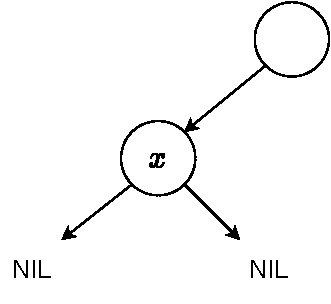
\includegraphics[scale=0.5]{img/del-leaf.ps}
  \caption{$x$ can be spliced out.} \label{fig:del-leaf}
\end{figure}

\begin{figure}[htbp]
  \centering
  \subcaptionbox{Before delete $x$.}{\includegraphics[scale=0.5]{img/del-lc-before.ps}}
  \subcaptionbox{After delete $x$, $x$ is spliced out, and replaced by its left child.}{\includegraphics[scale=0.5]{img/del-lc-after.ps}} \\
  \subcaptionbox{Before delete $x$.}{\includegraphics[scale=0.5]{img/del-rc-before.ps}}
  \subcaptionbox{After delete $x$, $x$ is spliced out, and replaced by its right child.}{\includegraphics[scale=0.5]{img/del-rc-after.ps}}
  \caption{Delete a node which has only one non-NIL child.}
  \label{fig:del-1child}
\end{figure}

\begin{figure}[htbp]
  \centering
  \subcaptionbox{Before delete $x$.}{\includegraphics[scale=0.5]{img/del-branch-before.ps}}
  \subcaptionbox{After delete $x$, $x$ is replaced by splicing the minimum element from its right child.}{ \includegraphics[scale=0.5]{img/del-branch-after.ps}}
  \caption{Delete a node which has both children.}
  \label{fig:del-branch}
\end{figure}

Based on this idea, the deletion can be defined as the below function.

\be
delete(T, x) = \left \{
  \begin{array}
  {r@{\quad:\quad}l}
  \phi & T = \phi \\
  node(delete(T_l, x), K, T_r) & x < k \\
  node(T_l, k, delete(T_r, x)) & x > k \\
  T_r & x = k \land T_l = \phi \\
  T_l & x = k \land T_r = \phi \\
  node(T_l, y, delete(T_r, y)) & otherwise
  \end{array}
\right .
\ee

Where
\[
\begin{array}{l}
T_l = left(T) \\
T_r = right(T) \\
k = key(T) \\
y = min(T_r)
\end{array}
\]

Translating the function to Haskell yields the below program.

\lstset{language=Haskell}
\begin{lstlisting}
delete Empty _ = Empty
delete (Node l k r) x | x < k = (Node (delete l x) k r)
                      | x > k = (Node l k (delete r x))
                      -- x == k
                      | isEmpty l = r
                      | isEmpty r = l
                      | otherwise = (Node l k' (delete r k'))
                          where k' = min r
\end{lstlisting}

Function \texttt{isEmpty} is to test if a tree is empty ($\phi$).
Note that the algorithm first performs search to locate the node
where the element need be deleted, after that it execute the
deletion. This algorithm takes $O(h)$ time where $h$ is the height
of the tree.

It's also possible to pass the node but not the element to the
algorithm for deletion. Thus the searching is no more needed.

The imperative algorithm is more complex because it need set the
parent properly. The function will return the root of the result tree.

\begin{algorithmic}[1]
\Function{Delete}{$T, x$}
  \State $r \gets T$
  \State $x' \gets x$ \Comment{save $x$}
  \State $p \gets $ \Call{Parent}{$x$}
  \If{\Call{Left}{$x$} $= NIL$}
    \State $x \gets $ \Call{Right}{$x$}
  \ElsIf{\Call{Right}{$x$} $= NIL$}
    \State $x \gets $ \Call{Left}{$x$}
  \Else
    \Comment{both children are non-NIL}
    \State  $y \gets $ \textproc{Min}(\Call{Right}{$x$})
    \State \Call{Key}{$x$} $\gets$ \Call{Key}{$y$}
    \State Copy other satellite data from $y$ to $x$
    \If{\Call{Parent}{$y$} $\neq x$}
      \Comment{$y$ hasn't left sub tree}
      \State \textproc{Left}(\Call{Parent}{$y$}) $\gets$ \Call{Right}{$y$}
    \Else
      \Comment{$y$ is the root of right child of $x$}
      \State \Call{Right}{$x$} $\gets$ \Call{Right}{$y$}
    \EndIf
    \If{\Call{Right}{$y$} $\neq NIL$}
      \State \textproc{Parent}(\Call{Right}{$y$}) $\gets$ \Call{Parent}{$y$}
    \EndIf
    \State Remove $y$
    \State \Return $r$
  \EndIf
  \If{$x \neq NIL$}
    \State \Call{Parent}{$x$} $\gets p$
  \EndIf
  \If{$p = NIL$}
    \Comment{We are removing the root of the tree}
    \State $r \gets x$
  \Else
    \If{\Call{Left}{$p$} $= x'$}
      \State \Call{Left}{$p$} $\gets x$
    \Else
      \State \Call{Right}{$p$} $\gets x$
    \EndIf
  \EndIf
  \State Remove $x'$
  \State \Return $r$
\EndFunction
\end{algorithmic}

Here we assume the node to be deleted is not empty (otherwise we can
simply returns the original tree). In other cases, it will first record
the root of the tree, create copy pointers to $x$, and its parent.

If either of the children is empty, the algorithm just splice $x$ out.
If it has two non-NIL children, we first located the minimum of right
child, replace the key of $x$ to $y$'s, copy the satellite data as
well, then splice $y$ out. Note that there is a special case that $y$
is the root node of $x$'s right sub tree.

Finally we need reset the stored parent if the original $x$ has only
one non-NIL child.
If the parent pointer we copied before is empty, it
means that we are deleting the root node, so we need return the new root. After
the parent is set properly, we finally remove the old $x$ from memory.

The relative Python program for deleting algorithm is given as below.
Because Python provides GC, we needn't explicitly remove the node
from the memory.

\lstset{language=Python}
\begin{lstlisting}
def tree_delete(t, x):
    if x is None:
        return t
    [root, old_x, parent] = [t, x, x.parent]
    if x.left is None:
        x = x.right
    elif x.right is None:
        x = x.left
    else:
        y = tree_min(x.right)
        x.key = y.key
        if y.parent != x:
            y.parent.left = y.right
        else:
            x.right = y.right
        if y.right is not None:
            y.right.parent = y.parent
        return root
    if x is not None:
        x.parent = parent
    if parent is None:
        root = x
    else:
        if parent.left == old_x:
            parent.left = x
        else:
            parent.right = x
    return root
\end{lstlisting}

Because the procedure seeks minimum element, it runs in $O(h)$ time on
a tree of height $h$.

\begin{Exercise}

\begin{itemize}
\item There is a symmetrical solution for deleting a node which has two
non-NIL children, to replace the element by splicing the maximum one out
off the left sub-tree. Write a program to implement this solution.
\end{itemize}

\end{Exercise}

\section{Randomly build binary search tree}
\index{binary search tree!randomly build}
It can be found that all operations given in this post bound to $O(h)$
time for a tree of height $h$. The height affects the performance
a lot. For a very unbalanced tree, $h$ tends to be $O(n)$, which leads
to the worst case. While for balanced tree, $h$ close to $O(\lg n)$.
We can gain the good performance.

How to make the binary search tree
balanced will be discussed in next post. However, there exists a simple
way. Binary search tree can be randomly built as described in \cite{CLRS}.
Randomly building can help to avoid (decrease the possibility) unbalanced
binary trees. The idea is that before building the tree, we can call a random
process, to shuffle the elements.

\begin{Exercise}

\begin{itemize}
\item Write a randomly building process for binary search tree.
\end{itemize}

\end{Exercise}

\section{Appendix: Example programs}

Definition of BST with parent field in C++.

\lstset{language=C++, frame=single}
\begin{lstlisting}
template<class T>
struct node {
    node(T x):key(x), left(nullptr), right(nullptr), parent(nullptr) {}

    ~node() {
        delete left;
        delete right;
    }

    node* left;
    node* right;
    node* parent; //可选,方便succ和pred操作
    T key;
};
\end{lstlisting}

Scheme/Lisp example program of insertion. It does not use pattern matching.

\lstset{language=lisp}
\begin{lstlisting}
(define (insert tree x)
  (cond ((null? tree) (list '() x '()))
	((< x (key tree))
	 (make-tree (insert (left tree) x)
		    (key tree)
		    (right tree)))
	((> x (key tree))
	 (make-tree (left tree)
		    (key tree)
		    (insert (right tree) x)))))
\end{lstlisting}

\begin{thebibliography}{99}

\bibitem{CLRS}
Thomas H. Cormen, Charles E. Leiserson, Ronald L. Rivest and Clifford Stein.
``Introduction to Algorithms, Second Edition''. ISBN:0262032937. The MIT Press. 2001

\bibitem{Bentley}
Jon Bentley. ``Programming Pearls(2nd Edition)''. Addison-Wesley Professional; 2 edition (October 7, 1999). ISBN-13: 978-0201657883

\bibitem{okasaki-blog}
Chris Okasaki. ``Ten Years of Purely Functional Data Structures''. http://okasaki.blogspot.com/2008/02/ten-years-of-purely-functional-data.html

\bibitem{sgi-stl}
SGI. ``Standard Template Library Programmer's Guide''. http://www.sgi.com/tech/stl/

\bibitem{literal-program}
http://en.literateprograms.org/Category:Binary\_search\_tree

\bibitem{wiki-fold}
http://en.wikipedia.org/wiki/Foldl

\bibitem{func-composition}
http://en.wikipedia.org/wiki/Function\_composition

\bibitem{curry}
http://en.wikipedia.org/wiki/Partial\_application

\bibitem{zipper-hbook}
Miran Lipovaca. ``Learn You a Haskell for Great Good! A Beginner's Guide''. the last chapter. No Starch Press; 1 edition April 2011, 400 pp. ISBN: 978-1-59327-283-8

\end{thebibliography}

\ifx\wholebook\relax\else
\end{document}
\fi
